\section{Spannungsreferenzen}

\begin{itemize}
    \item Referenzspannungsquellen liefern idealerweise Ausgangsspannungen, welche \textbf{unabhängig} von 
        Temperatur, Speisespannung und Last sind
    \item 2 Hauptprinzipien: Zenerdioden (meistens mit $V_{\rm Z} = 5.6 \,\volt$) und Bandgap-Quellen mit $V_{\rm out} = 1.25 \, \volt$
\end{itemize}


\subsection{Spanungsteiler}

\begin{minipage}[c]{0.2\columnwidth}
    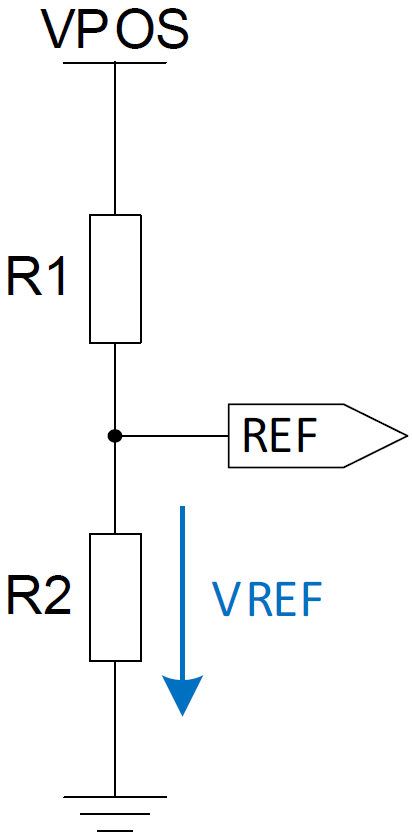
\includegraphics[width=\columnwidth]{images/spannungsteiler.png}
\end{minipage}
\hfill
\begin{minipage}[c]{0.78\columnwidth}
    \myul{\textbf{Speisespannungsabhängigkeit}}

        Spannungsänderung:
        $\boxed{\Delta V_{\rm ref} = \Delta V_{\rm POS} \frac{R_2}{R_1 + R_2}} $ \\
        Sensitivität:       
        $\boxed{ \overunderset{V_{\rm ref}}{V_{\rm POS}}{S} = \frac{\frac{\Delta V_{\rm ref}}{V_{\rm ref}}}{\frac{\Delta V_{\rm POS}}{V_{\rm POS}}} = 1 \text{ \textrightarrow\ schlecht}}$

    \vspace{0.2cm}
    \myul{\textbf{Temperaturabhängigkeit}} \\
    Da die Widerstände \textbf{gleiche Temperaturkoeffizienten} haben ändert sich der Strom durch $R_1$ und $R_2$, jedoch nicht das 
    Widerstandsverhältnis \textrightarrow\ $V_{\rm ref}$ bleibt \textbf{konstant} \textrightarrow\ gut

\end{minipage}

\myul{\textbf{Spannungsänderung bei Lastwechsel}}

\begin{minipage}[c]{0.2\columnwidth}
    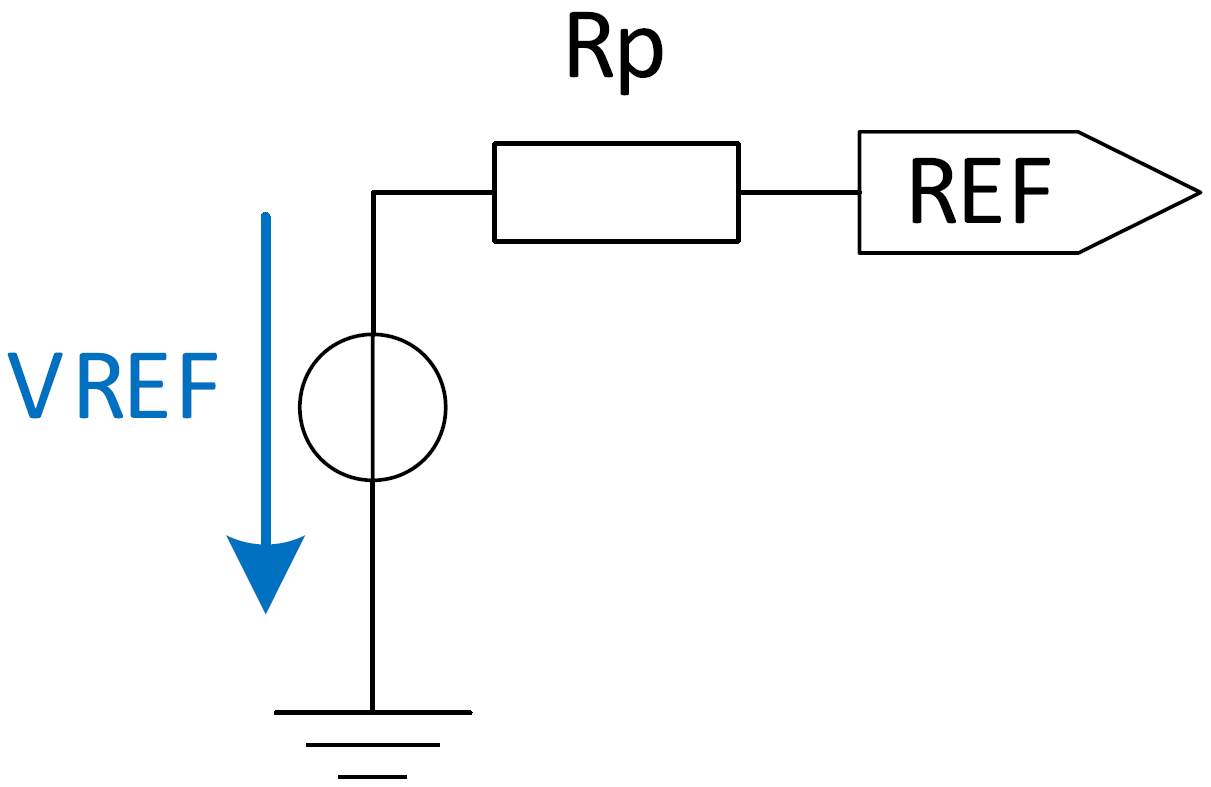
\includegraphics[width=\columnwidth]{images/thevenin.png}
\end{minipage}
\hfill
\begin{minipage}[c]{0.78\columnwidth}
    Ersatzschaltung der Referenzquelle durch Thévenin-Äquivalent mit
    $$ R_P = R_1 || R_2 \ \text{\textrightarrow\ sehr lastabhängig, da } R_P \text{ gross} $$
\end{minipage}


\subsection{Diodenreferenz}

    $$ \boxed{ V_{\rm ref} = V_D = n \cdot V_T \cdot \ln \Big( \frac{I}{I_S} \Big) 
    \quad \text{mit } V_T =\frac{k T}{q} \approx 25 \, \milli \ampere } $$
\begin{minipage}[c]{0.2\columnwidth}
    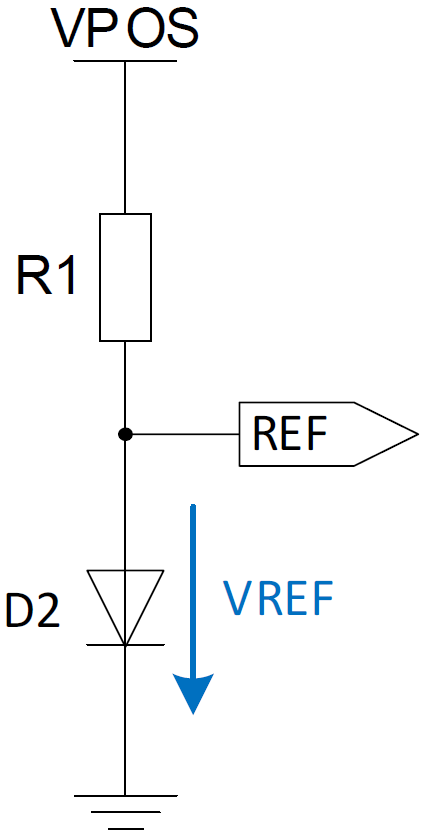
\includegraphics[width=\columnwidth]{images/diodenreferenz.png}
\end{minipage}
\hfill
\begin{minipage}[c]{0.78\columnwidth}
    %$$ I = \frac{V_{\rm POS} - V_D}{R_1} \approx \frac{V_{\rm POS}}{R_1} $$ % bei Platzproblemen weglassen

    \myul{\textbf{Speisespannungsabhängigkeit}}
    
    Sensitivität:
    $ \boxed{ \overunderset{V_{\rm ref}}{I}{S} = \frac{1}{\ln \Big( \frac{I}{I_S} \Big)} = 0.065 \text{ \textrightarrow\ gut }} $

    \vspace{0.2cm}
    \myul{\textbf{Temperaturabhängigkeit}} \\
    Diode hat einen \textbf{Temperaturkoeffizient von} $\boldsymbol{-2 \frac{\milli \volt}{\kelvin}}$, d.h. $V_{\rm ref}$ ändert ebenfalls
    mit ${-2 \frac{\milli \volt}{\kelvin}}$ \textrightarrow\ schlecht
\end{minipage}

\myul{\textbf{Spannungsänderung bei Lastwechsel}}

\begin{minipage}[c]{0.2\columnwidth}
    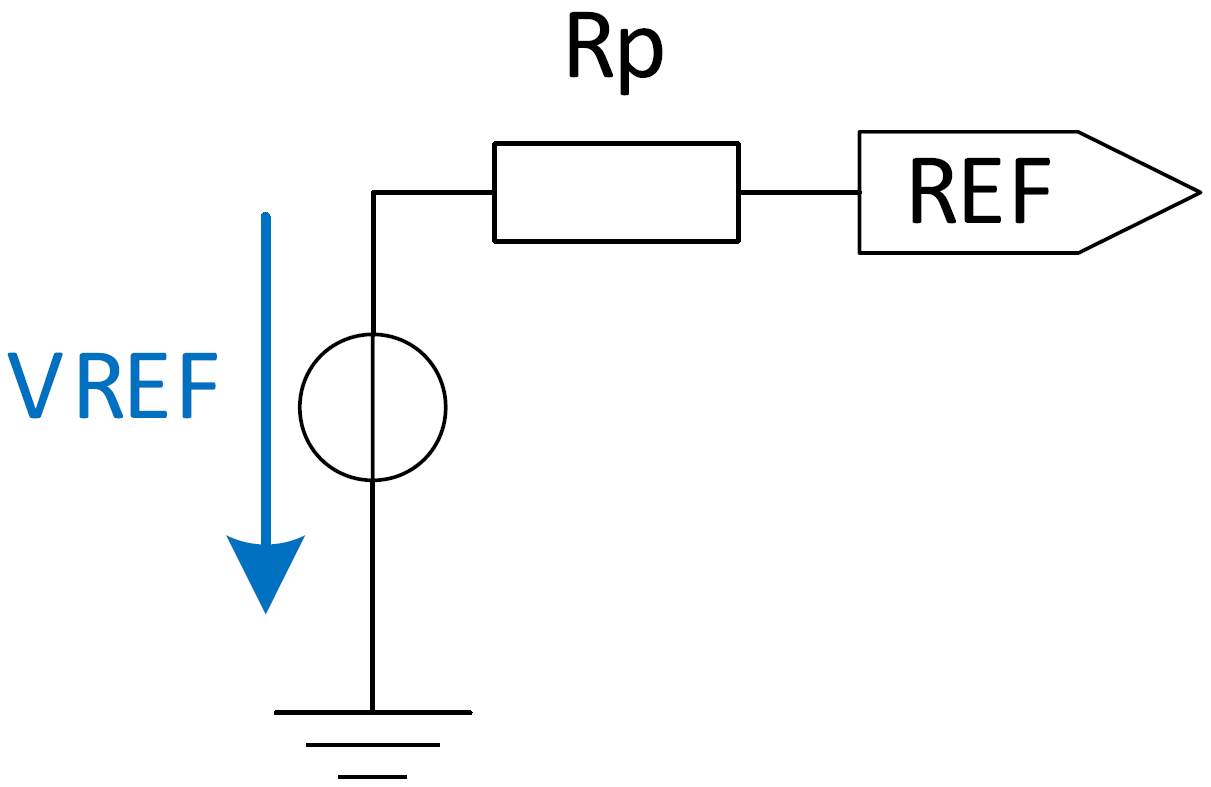
\includegraphics[width=\columnwidth]{images/thevenin.png}
\end{minipage}
\hfill
\begin{minipage}[c]{0.78\columnwidth}
    Diode durch Kleinsignal-Ersatzschaltung ersetzen und Ersatzschaltung der Referenzquelle durch Thévenin-Äquivalent mit
    $$ R_{\rm P} = R_1 || r_D \quad \text{\textrightarrow\ weniger lastabhängig, da } r_D = \frac{n \cdot V_T}{I_D} \approx 7 \, \ohm $$
\end{minipage}


\subsection{Spannungsreferenz mit mehreren Dioden}

\begin{minipage}[c]{0.25\columnwidth}
    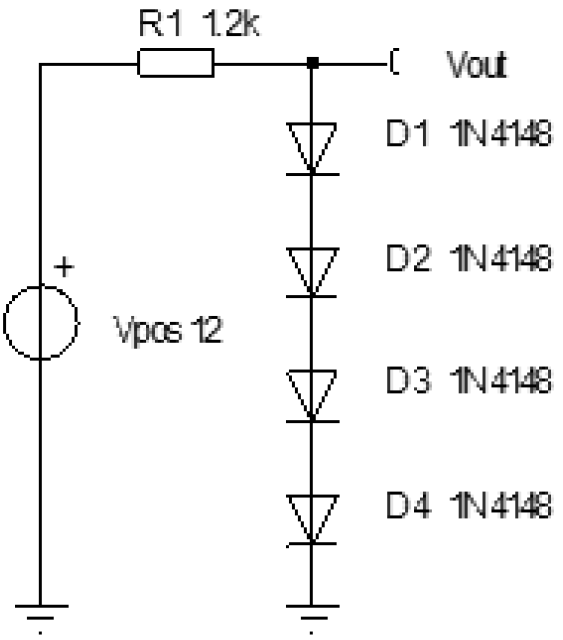
\includegraphics[width=\columnwidth]{images/spannungsreferenz_4_dioden.png}
\end{minipage}
\hfill
\begin{minipage}[c]{0.73\columnwidth}
    $m = $ Anzahl Dioden in Serie (links: $m = 4$) 

    \begin{itemize}
        \item Strom durch Dioden muss $> 0 \, \ampere$ sein, damit $V_D \approx 0.7 \, \volt$
        \item Spannung über $m$ Dioden: $ \boxed{ V_{\rm out} = m \cdot V_D }$
        \item Max. Ausgangsstrom: $ \boxed{I_{\rm out, max} =  \frac{V_{\rm pos} - V_{\rm out}}{R_1}} $
        \item \textbf{Temperaturabhängigkeit:} $TK_{\rm tot} = m \cdot -2 \frac{\milli \volt}{\kelvin}$
    \end{itemize}

\end{minipage}


\subsection{Spannungsreferenz mit Zenerdioden (Shunt-Regler)}

\textbf{Shunt-Regler:} Überflüssiger Strom wird durch ein Element abgeführt 
    \textrightarrow\ Je nach Last wird mehr oder weniger Strom in Z-Diode verheizt

\begin{minipage}[c]{0.15\columnwidth}
    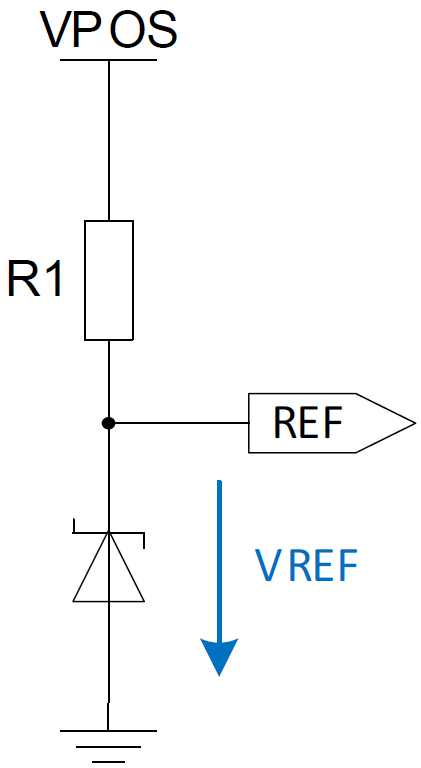
\includegraphics[width=\columnwidth]{images/spannungsreferenz_z-diode.png}
\end{minipage}
\hfill
\begin{minipage}[c]{0.78\columnwidth}
    \begin{itemize}
        \item $V_{\rm REF}$ entspricht Zener-Spannung der Z-Diode
        \item Häufigste Zener-Spannung: $5.6 \, \volt$ \textrightarrow\ TK $= 0 \frac{\milli \volt}{\kelvin}$
        \item Strom $I = \frac{V_{\rm POS} - V_{\rm REF}}{R_1}$ fliesst entweder durch Diode oder durch Last
        \item $I_{\rm out} < I_{\rm out, max} = \frac{V_{\rm POS} - V_{\rm REF}}{R_1}$
    \end{itemize}

\end{minipage}


\subsection[Bootstrap-Referenz (VD Stromquelle)]{Bootstrap-Referenz ($V_D$ Stromquelle)}

\begin{minipage}[c]{0.27\columnwidth}
    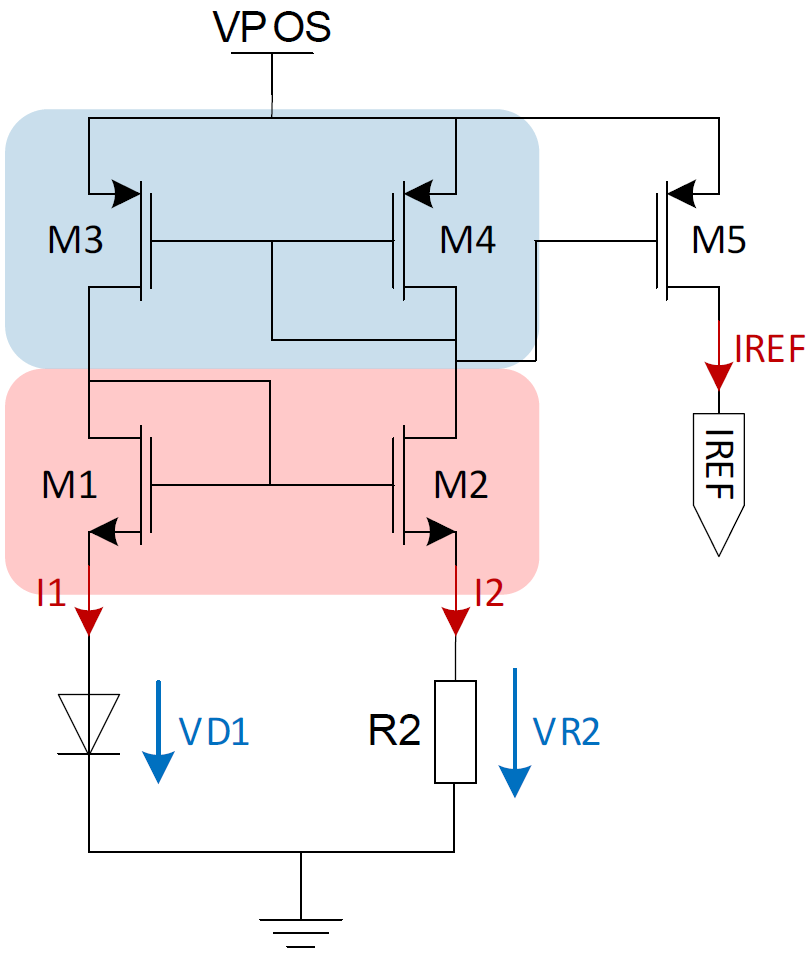
\includegraphics[width=\columnwidth]{images/bootstrap.png}
\end{minipage}
\hfill
\begin{minipage}[c]{0.71\columnwidth}
    \begin{itemize}
        \item Stromspiegel $M_3$ und $M_4$ \textrightarrow\ $I_1 = I_2$
        \item Stromspiegel $M_1$ und $M_2$ \textrightarrow\ $V_{\rm GS1} = V_{\rm GS1}$ da $I_1 = I_2$
        \item Da Temperaturkoeffizient von $V_{D1} \approx -2 \frac{\milli \volt}{\kelvin}$ nimmt $I_{\rm out}$ 
        mit steigender Temperatur ab \textrightarrow\ schlechte Referenz
        \item Schaltung hat zwei mögliche Arbeitspunkte\\
        (AP $I_1 = I_2 = 0$ ist unerwünscht!)
    \end{itemize}
\end{minipage}
$ \boxed{ V_{D1} = I_2 \cdot R_2 = V_{R2}} $ $ \boxed{ I_{\rm REF} = I_1 = I_2 } $


\subsection{Proportional To Absolute Temperature (PTAT)}

\begin{minipage}[c]{0.28\columnwidth}
    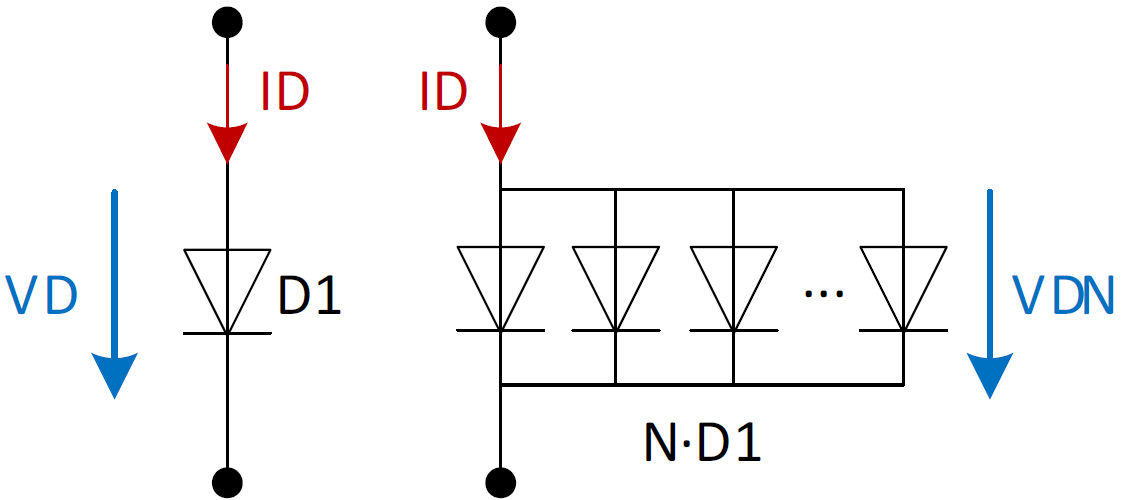
\includegraphics[width=\columnwidth]{images/ptat.png}
\end{minipage}
\hfill
\begin{minipage}[c]{0.7\columnwidth}
    \textrightarrow $\Delta V_T$ ist proportional zur absoluten Temperatur $T$
\end{minipage}

    \begin{tabular}{@{}c c@{}}
        $V_D = n \cdot \frac{k T}{q} \cdot \ln \Big( \frac{I_D}{I_S} \Big)$ & 
        $V_DN = n \cdot \frac{k T}{q} \cdot \ln \Big( \frac{I_D}{N \cdot I_S} \Big)$
    \end{tabular}

    $$ \boxed{ \Delta V_D = V_D - V_DN = n \cdot \frac{k T}{q} \cdot \ln(N)  = TK \cdot T }$$


\subsection{Bandgap-Spannungsreferenz}

\begin{minipage}[c]{0.2\columnwidth}
    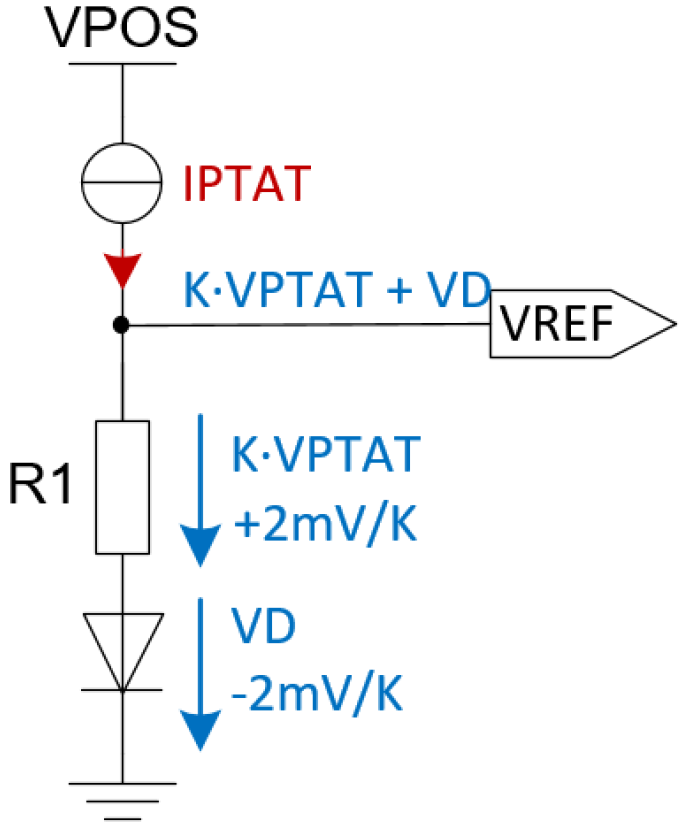
\includegraphics[width=\columnwidth]{images/bandgap_referenz.png}
\end{minipage}
\hfill
\begin{minipage}[c]{0.78\columnwidth}
    $$ \boxed{ V_{\rm REF} = K \cdot V_{\rm PTAT} + V_D } $$
    \begin{itemize}
        \item Der positive Temperaturkoeffizient von $V_{\rm PTAT}$ wird mit dem Faktor $K$ verstärkt, sodass 
            $K \cdot TK_{\rm PTAT} = +2 \frac{\milli \volt}{\kelvin}$
        \item Der nun positive Temperaturkoeffizient wird mit einer Diodenquelle mit $TK_{\rm Diode} = -2 \frac{\milli \volt}{\kelvin}$
            kompensiert
        \item Der gesamte Temperaturkoeffizient $TK_{\rm bandgap} = 0 \frac{\milli \volt}{\kelvin}$
        \item $V_{\rm REF}$ buffern, damit der Ausgang belastet werden darf
    \end{itemize}
\end{minipage}


\example{LM4041 Shunt Voltage Bandgap Reference}

\begin{minipage}[c]{0.25\columnwidth}
    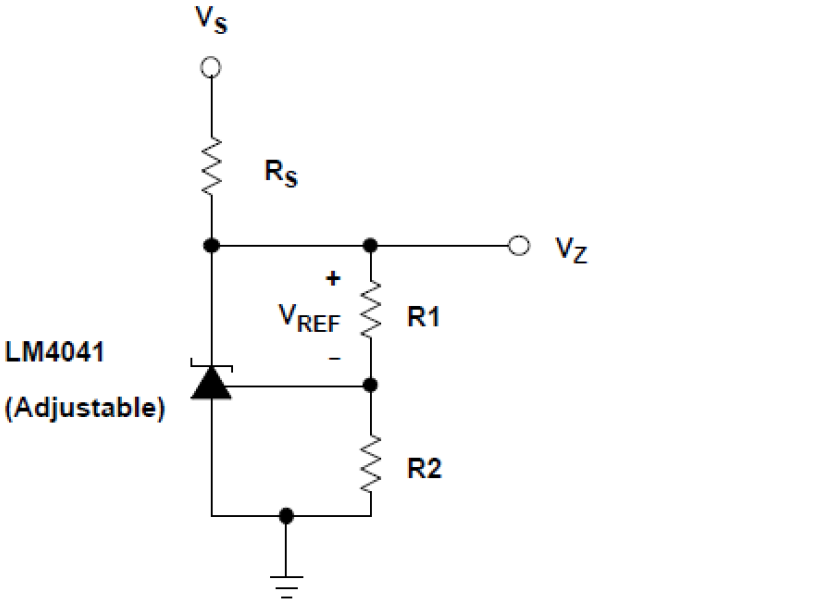
\includegraphics[width=\columnwidth]{images/beispiel_bandgap.png}
\end{minipage}
\hfill
\begin{minipage}[c]{0.72\columnwidth}
    $$ \boxed{ V_{\rm out} = V_Z = V_{\rm REF} \Big( 1 + \frac{R_2}{R_1} \Big) } $$
    \begin{itemize}
        \item Einstellbare Referenzspannung $V_Z = V_{\rm out}$
        \item Interne Referenz: $V_{\rm REF} = 1.25 \, \volt$ (Bandgap-Referenz)
    \end{itemize}
\end{minipage}

